\documentclass[11pt,a4paper]{article}
\usepackage[utf8]{inputenc}
\usepackage[portuguese]{babel}
\usepackage[T1]{fontenc}
\usepackage{inconsolata}
\usepackage{amsmath}
\usepackage{amsfonts}
\usepackage{amssymb}
\usepackage{graphicx}
\usepackage[left=2cm,right=2cm,top=2cm,bottom=2cm]{geometry}
\usepackage{listings}
\usepackage{xcolor}
\definecolor{backcolour}{rgb}{0.95,0.95,0.92}

\lstdefinestyle{mystyle}{
	tabsize = 4,
	basicstyle = \ttfamily,
	numbers = left,
	inputencoding=utf8,
    extendedchars=true,
	literate={á}{{\'a}}1 {ã}{{\~a}}1 {é}{{\'e}}1,
	showspaces=false,
    showstringspaces=false,
    showtabs=false,
    breaklines=true,
    breakatwhitespace=false,
    captionpos=b,
    keepspaces=true,
    numbersep=5pt
}
\lstset{style=mystyle}

\author{Alfredo Pacheco}
\title{Tarefa - MTF}
\date{}
\begin{document}

\maketitle

\lstinputlisting[language=Fortran]{../tarefa.f90}
\begin{figure}[p]
\centering
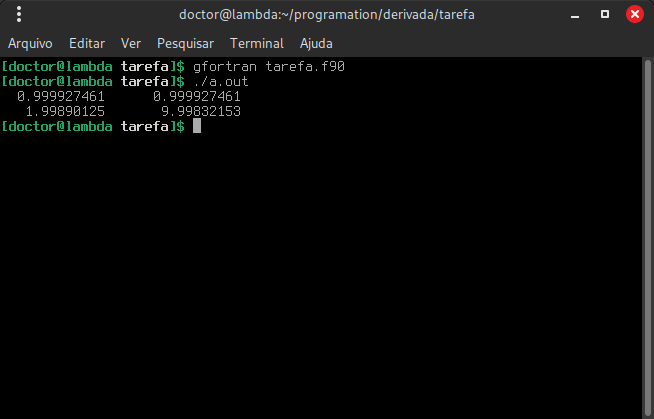
\includegraphics[width=\linewidth]{print.png}
\caption{Print do terminal com a execução do código.}
\end{figure}

\end{document}
